\documentclass[11pt,a4paper,oneside]{article}
\usepackage{graphicx}
\usepackage[usenames,dvipsnames]{xcolor}
\usepackage[section]{placeins}
\usepackage{fancyhdr}
\usepackage{hyperref}
\hypersetup{
    colorlinks,
    citecolor=RoyalBlue,
    filecolor=RoyalBlue,
    linkcolor=RoyalBlue,
    urlcolor=RoyalBlue
}
\usepackage[all]{hypcap}
\pagestyle{fancyplain}

\begin{document}
\lhead{Infographics Generator}
\rhead{Admin and User Manual}
\begin{titlepage}



\begin{center}


\includegraphics[width=1\textwidth]{images/sponsor-logo.png}\\[1cm]    

{ \huge \bfseries Infographics Generator}\\[0.4cm]
{ \large \bfseries Admin and User Manual}\\[0.4cm]

Louis Bodnar\\
Peter Chen\\
Lok Cheung\\
Kevin Shreve\\


\includegraphics[width=1\textwidth]{images/wrench3.png}\\   
\vfill

{\large \today}

\end{center}

\end{titlepage}

\tableofcontents
\newpage


\section{Admin Manual}
The Administrator manual is designed to assist in setting up the web service to a working status. Once this manual has been read in full, the product will be fully setup.\\

\subsection{Overview of System Architecture}
Below the system architecture diagram, gives a high level overview of the web application. This understanding is necessary to make sure that all setup and any modification is done within the right area of the code.\\

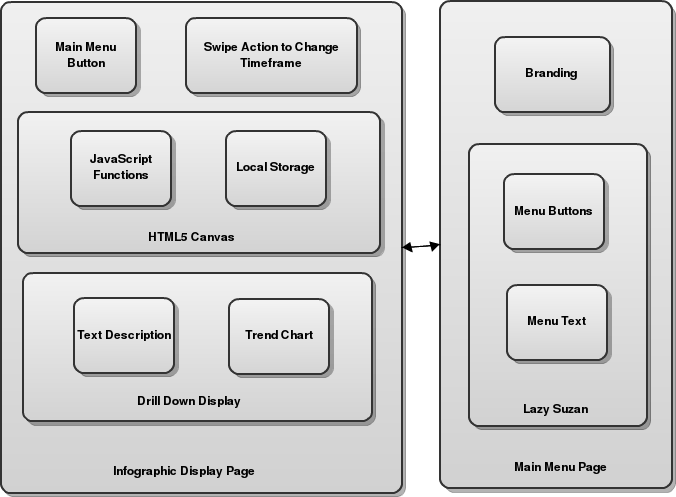
\includegraphics[width=.9\textwidth]{images/Capstone_-_System_Architecture_Diagram.png}\\   

\subsection{Database}
As the data is aggregated data from Urban Science and no calculations were necessary on our backend and therefore the data was just placed in a simple database with one table. The table has the following columns. {[}“record\_number”, “KPI\_Name”, “KPI\_Date”, “KPI\_Value”, “create\_dt”{]}. All of these columns all self explanatory, and follow what you would expect them too.\\

\subsection{Web Backend Setup}
For our server we setup a Windows Server 2008 Service pack two. Internet Information Services (IIS) Manager 6.0 (Build: 6002 Service Pack 2) was setup to host our website. All that was necessary on top of IIS was to install and enable all things for ASP.Net client to run successfully from the server.\\

\subsection{ASP.Net Script}
The ASP.Net Script that was created is named “KPI\_Handler.ashx”, this utilizes the class KPI.cs, which is an object that has all the same attributes as a database row. These two files are compiled and sit in the /bin/ folder at the same root as the web directory for the webapp. This enables the executables to be run upon request.\\

\subsection{Connecting the front and back ends}
A javascript function much like the code pasted below is all that is necessary to setup a new infographic page. The function LoadJSON(); is a function in “KPILocalStorage.js”. Once this function is called it uses jQuery (which at the time of this writing is version 1.7.1), to call the script in “KPI\_Handler.ashx”. The script creates a JSON serialized list and the jQuery call “\$.getJSON” takes each row and uses a helper function to store the data into the browser’s local storage.\\

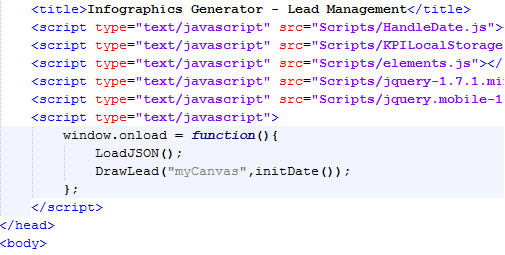
\includegraphics[width=.9\textwidth]{images/LoadJSON.png}\\   

\section{User Manual}
Navigation around the application is very simple and the user only is expected to know the following gestures, which is standard of a mobile application.\\

\subsection{Swipe} 
Both on the homepage (index.html), and on each individual infographic pages (lead.html, sales.html, service.html the user is expected to know to swipe. On the homepage they must swipe in order to turn the lazy susan menu selector to select a new infographic category. The image below shows how a user can use the swipe gesture on the homepage. A user may also do the swipe gesture to change the month of data that is being displayed. \\

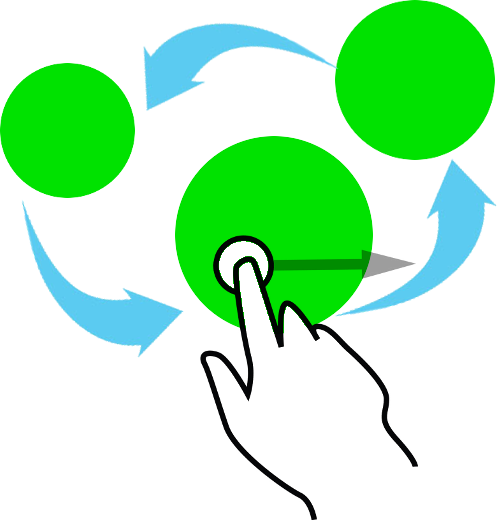
\includegraphics[width=.9\textwidth]{images/switcheroo.png}\\   

\subsection{Tap}
The tapping feature is used in multiple places around the infographic. On the homepage a user may tap on an icon in the foreground to choose to view that categories data. A user may also tap an icon in the background to bring it to the foreground. From within an infographic a user can use the tap to select the home button to navigate back to the homepage or tap an infographic element to bring up the drill down display. The image below gives a visual representation of the what action the user must complete to bring up the drill down display.\\

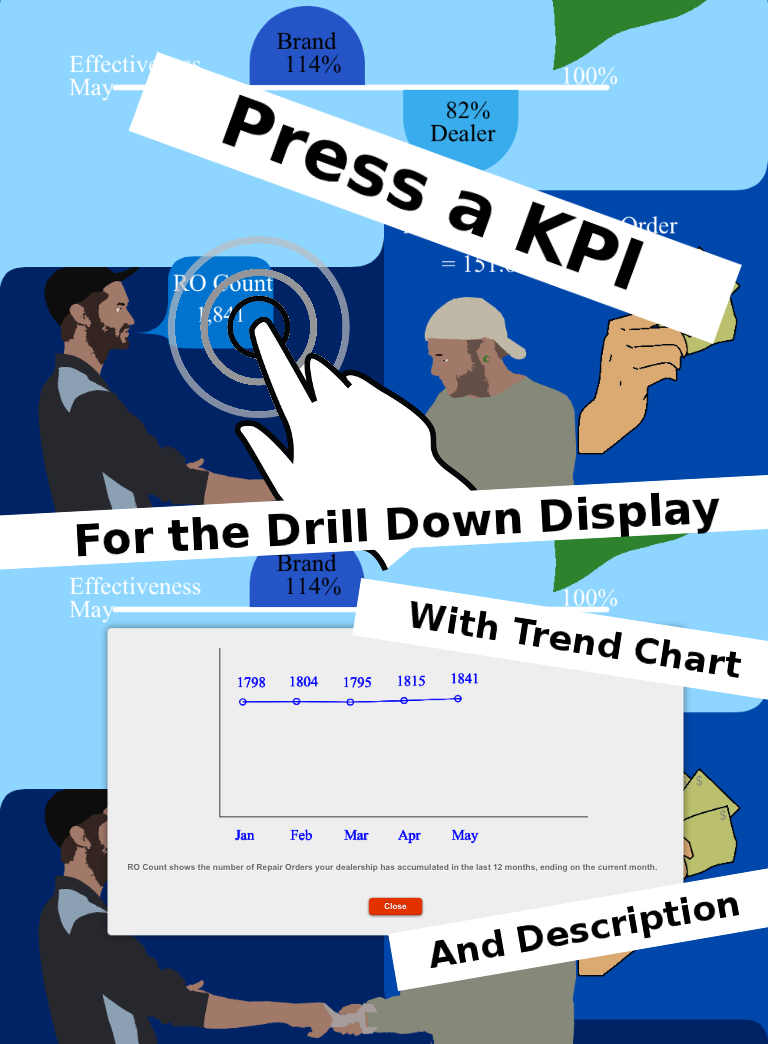
\includegraphics[width=.9\textwidth]{images/fun.png}\\   

\subsection{Scroll}
Scrolling is when a user presses on the iPad and then slides their finger up or down. This is a typical feature that users should be accustomed to using as it has the same functionality as Safari on the iPad typically does. The image below further clarifies this.\\

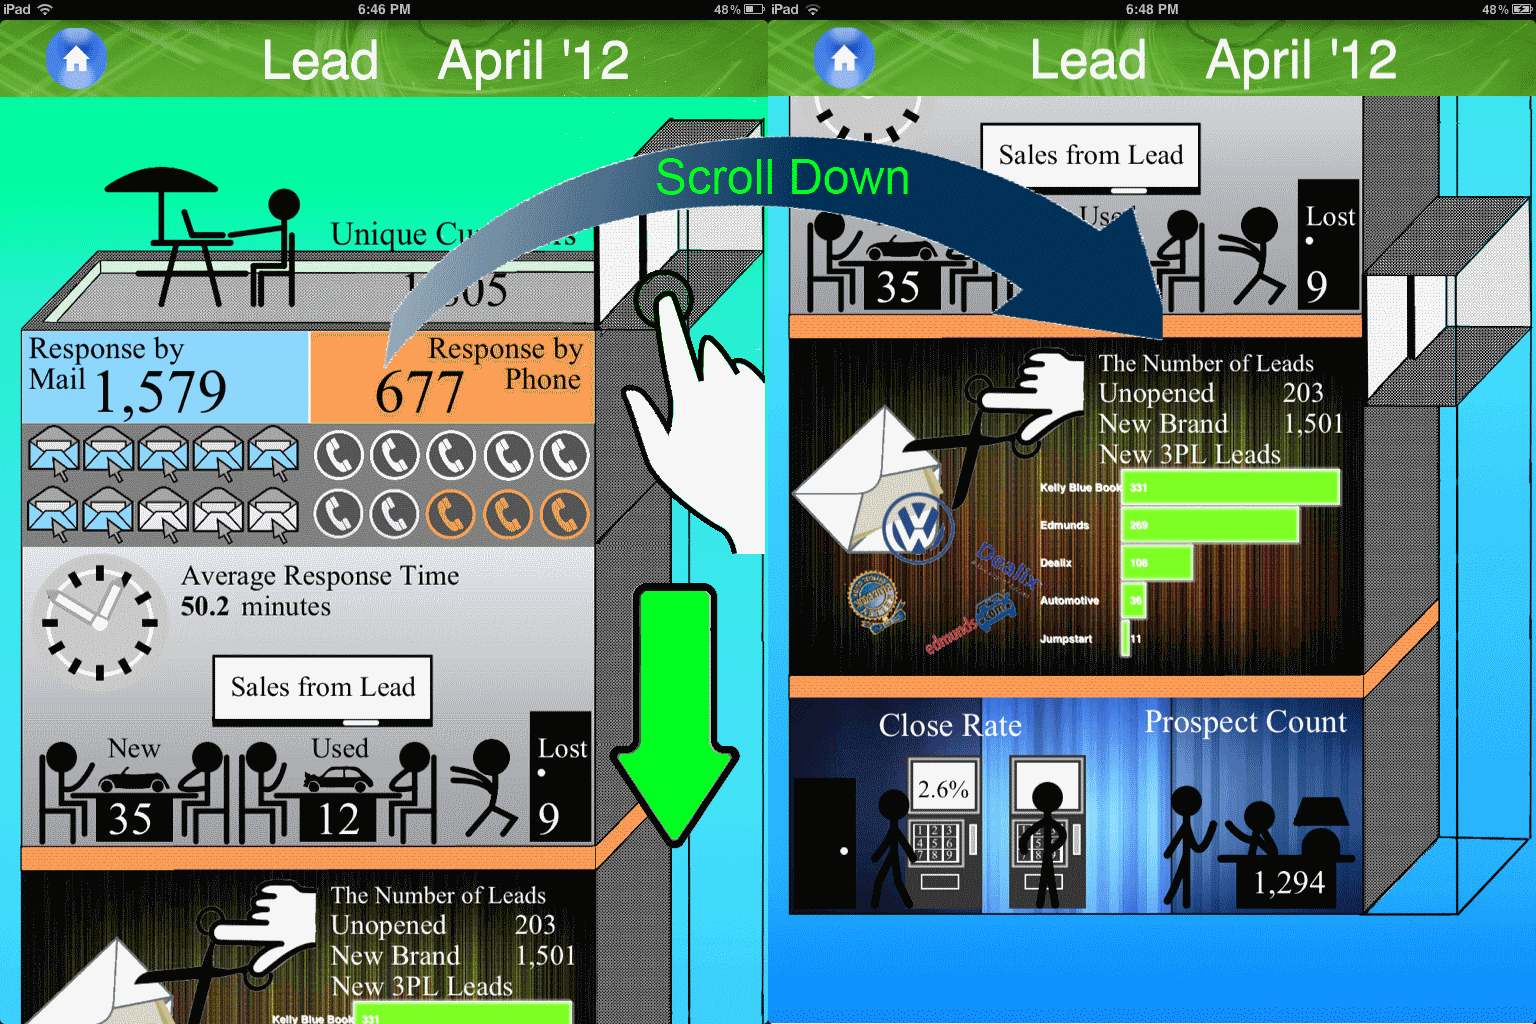
\includegraphics[width=1\textwidth]{images/IMG_02.png}\\   

\end{document}
